\section{Methodische Vorgehensweise}
\subsection{Datenerhebung}
Für die Gegenüberstellung der Technologietrends in der akademischen Forschung und praktizierenden Wirtschaft werden, wie bereits in Abschnitt \ref{sec:method} erwähnt, zwei Arten von Quellen herangezogen.

\subsubsection{Gartner Hype Cycle for Emerging Technologies}\label{sec:ghcet}
Der \glqq Gartner Hype Cycle for Emerging Technologies\grqq~repräsentiert als markt\-führendes Beratungsunternehmen für Technologieprognosen den Part der praktizierenden Wirtschaft. Dabei dienen die Technologien in der Phase \glqq Peak of Inflated Expectations\grqq~in vorliegender Reihenfolge als Datenbasis für die Analyse, da sie den Höhepunkt der Trendwahrnehmung darstellen.

Eine komplette Ausgabe inklusive der Erläuterungen einzelner Phasen sowie der aufgeführten Technologien ist kostenpflichtig über den Webauftritt des Unternehmens: \url{https://www.gartner.com} erhältlich. Für die vorliegende Untersuchung ist sie jedoch nicht erforderlich, da die notwendigen Informationen in Unterpfaden der Webseite frei erhältlich sind.

Die graphische Darstellung des \glqq Hype Cycle for Emerging Technologies \grqq~wird jährlich in Form eines Nachrichtenartikels frei veröffentlicht.\footnote{\citeNP<Vgl.>[o.S.]{ghcet2016}}
Die genaue Aufteilung der Technologien in die fünf bekannten Phasen ist wiederum der Webseite, wo der Artikel gekauft und heruntergeladen werden kann, aus dem dort aufgeführten Inhaltsverzeichnis zu entnehmen.\footnote{\citeNP<Vgl.>[o.S.]{ghc2016}}

Für die optimale Ausrichtung der Analyse an die Leitfragen ist es sinnvoll, eine relativ aktuelle Ausgabe des \glqq Hype Cycle\grqq~zu verwenden, nicht jedoch die neuste. Denn für die Leitfrage L3 wird mindestens eine neuere Ausgabe als die analysierte benötigt. Bei zu alten Publikationen besteht wiederum die Gefahr, dass durch gegenseitige Einflussnahme eine Angleichung bspw. der Begrifflichkeiten die Ergebnisse verfälschen könnte.

Die aktuellste Ausgabe des \glqq Gartner Hype Cycle for Emerging Technologies\grqq~ ist im Juli 2017 erschienen.\footnote{\citeNP<Vgl.>[o.S.]{ghc2017}} Deshalb fällt die Wahl auf die unmittelbar vorausgegangene Veröffentlichung aus dem Jahre 2016. In der Phase \glqq Peak of Inflated Expecta\-tions\grqq~sind folgende Technologien aufgeführt:\footnote{\citeNP<Vgl.>[o.S.]{ghc2016}}

\begin{itemize}
	\item Gesture Control Devices
	\item Micro Data Centers
	\item Smart Robots
	\item Blockchain
	\item Connected Home
	\item Cognitive Expert Advisors
	\item Machine Learning
	\item Software-Defined Security
	\item Autonomous Vehicles
	\item Nanotube Electronics
	\item Software-Defined Anything (SDx)
\end{itemize}

In Abbildung \ref{fig:ghc2016} ist der dazugehörige Graph zu sehen, dem zusätzlich die Erwartungen an die Technologie in Abhängigkeit zum Reifegrad sowie die voraussichtliche Dauer bis zur Erreichung des \glqq Plateau of Productivity\grqq~entnommen werden können.

\begin{figure}[ht]
	\centering
	\caption{Gartner Hype Cycle for Emerging Technologies, 2016}
	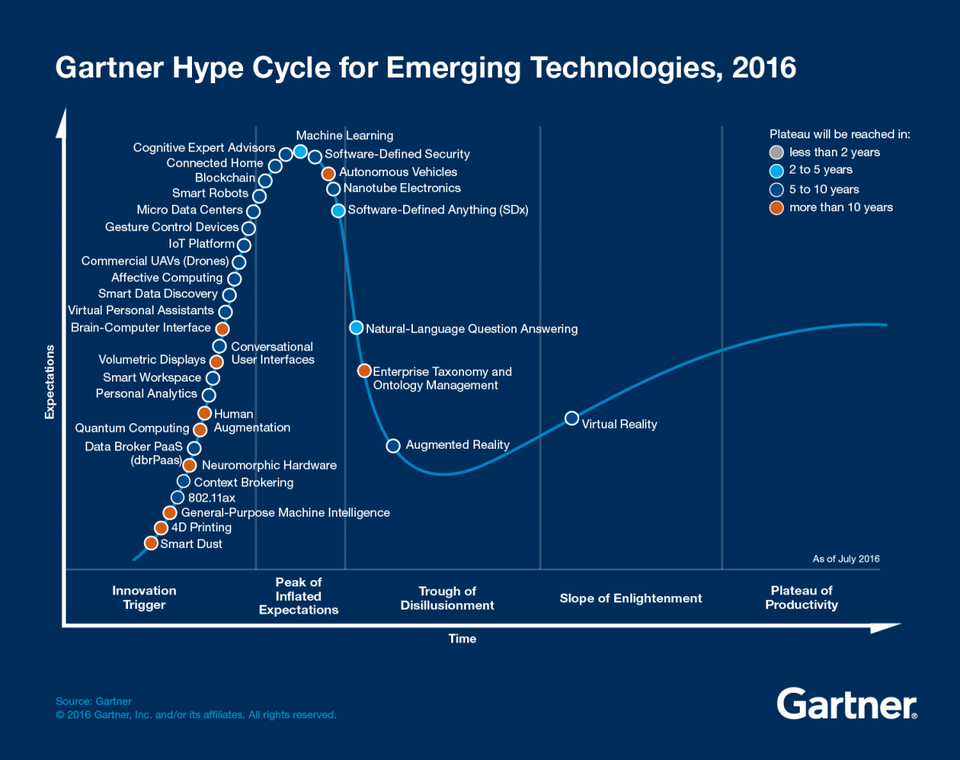
\includegraphics[width=0.9\linewidth]{img/Hype_Cycle_2016.jpg}
	\caption*{\protect\citeNP<Quelle:>[o.S.]{ghcet2016}}
	\label{fig:ghc2016}
\end{figure}

Demnach waren beispielsweise die Erwartungen und somit die Trendwahrnehmung für die Technologie \glqq Machine Learning\grqq~im Jahre 2016 am höchsten. Die Technologien links davon hatten eine geringere Reife, die rechts davon eine höhere. Insgesamt handelt es sich bei den Technologien allesamt um Trends des Jahres 2016 in der praktizierenden Wirtschaft.

Um den Trendverlauf der ausgewählten Technologien zu bestimmen, müssen weitere \glqq Hype Cyles\grqq~betrachtet werden. Das erstmalige Erscheinen in einer Publikation liefert einen Hinweis darauf, wann eine Technologie die Aufmerksamkeit der relevanten Gruppe von praktizierenden Wirtschaftlern erlangt hat. Die Verteilung der Vorkommnisse und Abwesenheiten der Technologien in den jeweiligen Ausgaben ermöglicht Rückschlüsse über den Zeitraum und Verlauf der Trendwahrnehmung.

Zur Ermittlung des erstmaligen Erscheinens werden solange vergangene \glqq Hype Cycles\grqq~betrachtet, bis die jeweils gesuchte Technologie in einer vorhergehenden Ausgabe fehlt. Für die meisten Technologien ist damit das Jahr der ersten Ausgabe ermittelt. Ist die Prognose der Dauer bis zum Erreichen des \glqq Plateaus\grqq~ mit größer als fünf Jahren angegeben, sind weitere Vorgänger zu betrachten, da eine Technologie in der Zeit vorübergehend unter die Trendschwelle fallen kann.

Für die Ermittlung des Trendverlaufs wird zusätzlich die aktuelle Ausgabe hinzugenommen.

Dabei sind folgende Parameter für die Auswertung festzuhalten:

\begin{enumerate}
	\item Name der Technologie
	\item Jahr aller Erscheinungen mit Zuordnung zur jeweiligen Phase
	\item Position innerhalb der entsprechenden Phase
\end{enumerate}

\subsubsection{Literaturdatenbanken}\label{sec:lit_data}
Demgegenüber wird die Datenbasis der akademischen Forschung aus Abfragen in relevanten Literaturdatenbanken erhoben. Aufgrund ihrer hohen Abdeckung wissenschaftlich, technologischer Publikationen werden folgende Datenbanken durchsucht:
\begin{description}
	\item [WoS:] Web of Science Core Collection - \url{http://apps.webofknowledge.com}
	\item [IEEE:] IEEE Xplore Digital Library - \url{https://ieeexplore.ieee.org}
	\item [ACM:] The ACM Guide to Computing Literature - \url{https://dl.acm.org}
\end{description}

Diese enthalten neben den in Abschnitt \ref{sec:acad_pub} genannten Fachzeitschriften und Konferenzbeiträgen weitere Formen von Veröffentlichungen, wie beispielsweise Bücher oder Standards. Daher ist die Suche ausschließlich darauf einzugrenzen, wobei die Ergebnisse nach Veröffentlichungsform getrennt voneinander gehalten werden, da dies genauere Rückschlüsse über den tatsächliche Verlauf ermöglicht.

Alle Suchmaschinen sind im erweiterten Suchmodus mit vergleichbarer Funktionalität zur Vergabe von Suchkriterien ausgestattet. Diese sind gezielt einzusetzen, damit das Suchergebnis einerseits möglichst vollständig ist und andererseits keine \glqq False Positives\grqq~liefert. Deshalb beschränkt sich die Suche der Technologien auf die Metadaten Titel, Stichwörter und Abstract einer Publikation.

Der erweiterte Suchmodus bietet in allen Suchmaschinen die Möglichkeit, Suchanfragen mittels Kommandoanweisungen einzugeben. Die Operatoren zur Verknüpfung von Suchbegriffen sind nahezu identisch, wobei die Syntax einer Suchanweisung teilweise unterschiedlich ist. Somit sind die Querys untereinander nicht wahllos austauschbar.

Bei IEEE und ACM können einige Suchkriterien wie beispielsweise die Veröffentlichungsform nicht als Teil des Querys formuliert werden. Es werden alternativ Bedienelemente in der Web\-oberfläche angeboten, mit denen die Suche entsprechend eingegrenzt werden kann. Da die Auswahl dieser Suchkriterien bei einem HTTP-Request als \glqq Query Strings\grqq~an die GET-Methode übergeben werden, ist die Eingrenzung auch über die Modifikation der URL möglich.

Im ersten Schritt werden die Technologien aus Abschnitt \ref{sec:ghcet} unverändert in die Suchmaschine eingegeben, um einen ersten Eindruck der Datenlage im Hinblick auf potentielle Unterschiede bei den Begrifflichkeiten zu erhalten. Mit den oben genannten Eingrenzungen ergibt das für den Begriff \glqq Machine Learning\grqq~in Fachzeitschriften folgende Suchalgorithmen je Suchmaschine:

\begin{description}
	\item [WoS:] \begin{verbatim}
	(TS=("machine learning")) AND DOCUMENT TYPES: (Article)
	\end{verbatim}

	\item [IEEE:] \begin{verbatim}
	("machine learning")
	\end{verbatim}
	Zusätzliche Filtereinstellungen:
	\begin{itemize}
		\item Search Context: Metadata only
		\item Content Types: Journals \& Magazines
	\end{itemize}

	\item [ACM:] \begin{verbatim}
	acmdlTitle:(+"machine learning") OR
	recordAbstract:(+"machine learning") OR
	keywords.author.keyword:(+"machine learning")
	\end{verbatim}
	Zusätzliche Filtereinstellung:
	\begin{itemize}
		\item Refine by Publications / All Publications / Periodical
	\end{itemize}
\end{description}

Für die Ermittlung der idealen Suchalgorithmen ist es wichtig, die im \glqq Hype Cycle\grqq~vorkommenden Technologiebegriffe genau zu verstehen. Dies gilt insbesondere, wenn diese mit der wissenschaftlichen Benennung nicht exakt übereinstimmen. Deshalb werden die Technologien zunächst in Gartners IT-Glossar\footnote{\url{https://www.gartner.com/it-glossary/}} verifiziert.

Im nächsten Schritt gilt es, alternative Bezeichnungen der Technologiebegriffe aus dem \glqq Hype Cycle\grqq~herauszufinden, um eine möglichst vollständige Abdeckung von Publikationen zu den entsprechenden Technologien zu erhalten. Dazu werden die Stichwörter\footnote{engl. keywords} der einzelnen Suchergebnisse stichprobenartig nach Synonymen durchsucht, welche anschließend adjunktiv mit der ursprünglichen Suche verknüpft werden.

Andersherum sind Begriffe auszuschließen, die für eine höhere Evolutionsstufe der ursprünglichen Technologie stehen, diese jedoch signifikant erweitern, so dass ein neuer Begriff einen neuen Kontext rechtfertigt. Ein Beispiel dafür sind die Technologien \glqq Machine Learning\grqq~und \glqq Deep Learning\grqq, welche jeweils ihre eigene Daseinsberechtigung haben und daher in der aktuellen Ausgabe des \glqq Hype Cycle for Emerging Technologies 2017\grqq~im \glqq Peak of Inflated Expectations\grqq~nebeneinander stehen.\footnote{\citeNP<Vgl.>[S.~45.]{ghc2017}} Da es sich bei \glqq Deep Learning\grqq~um die neuere Technologie handelt, wird sie mit dem exkludierenden Operator \glqq NOT\grqq~jeweils herausgenommen.

TODO: Suchalgorithmen

Für die Auswertung wird die Menge der Publikationen pro Jahr und Filter benötigt. Dazu werden die entsprechenden Exportfunktionen der jeweiligen Suchmaschinen eingesetzt. Im WoS ist ein Export der Verteilung von Publikationen pro Jahr von maximal \numprint{200000} Datensätzen mit einer einzigen Anweisung im TSV-Format (Tabulator-Seperated Values) möglich.

Die anderen beiden Suchmaschinen erlauben lediglich einen Export von maximal \numprint{2000} Datensätzen der Metadaten -- inklusive Abstracts, Stichwörter etc. -- im CSV-Format (Comma-Seperated Values). Das bedeutet, dass für Suchergebnisse mit mehr als \numprint{2000} Ergebnissen mehrere Exportanweisungen mit jeweils abgrenzbaren Filterkriterien durchzuführen sind, um Redundanzen in einzelnen Exportvorgängen auszuschließen. Ein geeignetes Mittel dazu ist die Eingrenzung der Suchergebnisse nach Veröffentlichungs\-zeiträumen mit jeweils kleiner gleich \numprint{2000} Ergebnissen. Die einzelnen Dateien sind anschließend zusammenzuführen.

Für Technologien mit mehreren Tausend Such\-ergebnissen bedeutet dies allerdings, dass die zusammengeführten Dateien sehr groß werden. Der Export einer Datei mit \numprint{2000} Einträgen aus dem IEEE ist beispielsweise um die 4 Megabyte groß und dauert knapp eine Minute. Für den Begriff \glqq Machine Learning\grqq~mit mehr als \numprint{50000} Ergebnissen ist daher die genannte Vorgehensweise nicht praktikabel. Insbesondere auch deshalb, da aus den exportierten Daten allein die Veröffentlichungsjahre für die Analyse verwendet werden. In solchen Fällen wird der \glqq Query String\grqq~der URL des \glqq HTTP-Requests\grqq~modifiziert, um die Suche auf einzelne Jahre einzugrenzen und die Anzahl der Publikationen pro Jahr direkt abzulesen.

Demgegenüber wird die Anzahl aller Publikationen in dem Betrachtungszeitreim pro Suchmaschine und Veröffentlichungsform ermittelt, um eine Vorstellung über die Dimension der Publikations\-aktivitäten zu gewinnen. Dies geschieht ebenfalls über URL-Modifikationen; das Ergebnis wird tabellarisch aufbereitet.

\subsection{Operationalisierung der Daten}
Im nächsten Schritt werden die gewonnenen Daten strukturiert, um die Gegenüberstellung der Technologietrends in Wirtschaft und Wissenschaft im Hinblick auf die Beantwortung der Leitfragen zu ermöglichen.

Da zur Trendbestimmung auf wissenschaftlicher Seite die Anzahl an Publikationen verwendet wird, sind auf Seiten des \glqq Hype Cycles\grqq~alle Indikatoren einzubeziehen, die das Skalenniveau daran angleichen.

Der Trendverlauf in der akademischen Forschung wird maschinell ausgewertet, daher werden die Export-Dateien mithilfe von Python-Skripten in ein einheitliches CSV-Format überführt, welches aus den beiden Spalten \glqq Veröffentlichungsjahr\grqq~und \glqq Anzahl der Veröffentlichungen\grqq~besteht.

Für die Darstellung im Text werden entsprechende Repräsentationsformen wie Kurven und Tabellen verwendet.

\subsubsection{Verteilung der Technologietrends in der praktizierenden Wirtschaft}
Nachdem die zeitliche Verteilung der Technologien aus Abschnitt \ref{sec:ghcet} ermittelt ist, wird eine Übersicht darüber inklusive weiterer relevanter Daten erstellt. Aus Gründen der Vergleichbarkeit mit der Verteilung der wissenschaftlichen Publikationen eignet sich dazu eine Tabellenform, in der die Technologien in ihrer ursprünglichen Reihenfolge als Zeilenüberschriften und die Veröffentlichungsjahre als Spaltenüberschriften dienen, wie in Tabelle~\ref{tab:dist_ghc} zu sehen ist. Die Technologien werden dabei durch ihre Akronyme abgekürzt, da sie in vorliegendem Fall eindeutig sind und die Übersichtlichkeit der Tabelle erhöhen.

Leere Zellen bedeuten, dass die Technologie im entsprechenden Veröffentlichungsjahr nicht vorkommt. Anderenfalls setzt sich der Eintrag prinzipiell aus zwei Teilen zusammen. Im ersten Teil wird das Kürzel der Phase des \glqq Hype Cyles\grqq~aufgeführt, in der die Technologie vorkommt. Für vorliegende Datenbasis werden folgende Kürzel benutzt:

\begin{description}
	\item[I:] Innovation Trigger
	\item[P:] Peak of Inflated Expectations
	\item[T:] Trough of Disillusionment
\end{description}

Die anderen beiden Phasen bleiben unberücksichtigt, da sie die zu untersuchenden Technologien in keiner Ausgabe enthalten. Der zweite Teil gibt die Position der Technologie unter allen anderen der jeweiligen Phase wieder.

Durch Hinzunahme von Indikatoren zur Gewichtung wird somit das Skalenniveau der Daten erhöht, um sie mit den Daten der Forschung besser vergleichen zu können.

Für die Technologie \glqq Machine Learning\grqq~im Jahre 2016 heißt das bspw., dass sie in der Phase \glqq Peak of Inflated Expectations\grqq~erschienen ist, insgesamt elf Technologien in dieser Phase vorkommen und \glqq Machine Learning\grqq~an Position sieben zu finden ist. Zusätzlich wird die Spalte des zugrundeliegenden Jahres mit einem Sternchen~(*) gekennzeichnet, falls es sich bei der Technologie um den höchsten Punkt der Kurve handelt.

\begin{table}
	\caption{Verteilung der Technologien des \glqq Gartner Hype Cycle\grqq}
	\centering
	\label{tab:dist_ghc}
\begin{tabularx}{\linewidth}{X|XXXXXXX}
	Techn. & 2010 & 2012 & 2013 & 2014 & 2015 & 2016 & 2017 \\
	\hline
	GCD &  &  &  &  &  & P 1/11 &  \\
	\hline
	MDC &  &  &  &  & P 2/10 & P 2/11 &  \\
	\hline
	SR &  &  &  & I 13/17 & I 11/18 & P 3/11 & P 3/13 \\
	\hline
	B &  &  &  &  &  & P 4/11 & P 12/13 \\
	\hline
	CH &  &  &  & I 5/17 & I 13/18 & P 5/11 & P 6/13 \\
	\hline
	CEA &  &  &  &  &  & P 6/11 & T 1/4 \\
	\hline
	ML &  &  &  &  & P 8/10 & P 7/11* & P 8/13 \\
	\hline
	SDS &  &  &  &  & I 18/18 & P 8/11 & T 3/4 \\
	\hline
	AV & I 7/12 & I 7/9 & I 12/14 & P 3/10 & P 5/10* & P 9/11 & P 9/13 \\
	\hline
	NE &  &  &  &  &  & P 10/11 & P 10/13 \\
	\hline
	SDx &  &  &  &  &  & P 11/11 &  \\
\end{tabularx}
\caption*{Quelle: Eigene Darstellung}
\end{table}

\subsubsection{Verteilung der Technologietrends in der wissenschaftlichen Forschung}
Um die Dimension der Kennzahlen von wissenschaftlichen Veröffentlichungen besser einordnen zu können, wird zunächst einmal eine tabellarische Übersicht über alle Veröffentlichungen des Betrachtungszeitraumes erstellt. Tabelle \ref{tab:dist_full_pub} stellt die Veröffentlichungsjahre mit den Suchmaschinen sowie Veröffentlichungsformen gegenüber und listet dazu die jeweilige Anzahl auf.

\begin{table}
	\caption{Gesamtveröffentlichungen von Artikeln und Konferenzbeiträgen der Jahre 2010-2018}
	\centering
	\label{tab:dist_full_pub}
\begin{tabularx}{\linewidth}{XXXXXXX}
	\hline 
	\multirow{2}{*}{Jahr} & \multicolumn{2}{c}{WoS} &  \multicolumn{2}{c}{IEEE}  &  \multicolumn{2}{c}{ACM}  \\ 
	& Artikel & Konf. & Artikel & Konf. & Artikel & Konf. \\ 
	\hline 
	2010 & \numprint{1186641} & \numprint{49975} & \numprint{36936} & \numprint{219692} & \numprint{57422} & \numprint{91322} \\ 
	2011 & \numprint{1262629} & \numprint{37324} & \numprint{39922} & \numprint{209425} & \numprint{56329} & \numprint{83948} \\ 
	2012 & \numprint{1322862} & \numprint{27633} & \numprint{42104} & \numprint{188042} & \numprint{55872} & \numprint{80413} \\ 
	2013 & \numprint{1396999} & \numprint{25583} & \numprint{44864} & \numprint{179732} & \numprint{53039} & \numprint{61839} \\ 
	2014 & \numprint{1436384} & \numprint{21879} & \numprint{46983} & \numprint{186662} & \numprint{53174} & \numprint{54270} \\ 
	2015 & \numprint{1673986} & \numprint{31740} & \numprint{50212} & \numprint{195474} & \numprint{58006} & \numprint{58235} \\ 
	2016 & \numprint{1743515} & \numprint{35747} & \numprint{53082} & \numprint{203381} & \numprint{63321} & \numprint{35803} \\ 
	2017 & \numprint{1796767} & \numprint{33951} & \numprint{58098} & \numprint{202134} & \numprint{55052} & \numprint{28942} \\ 
	2018 & \numprint{1082773} & \numprint{20702} & \numprint{42094} & \numprint{47429} & \numprint{21483} & \numprint{15720} \\ 
	\hline 
\end{tabularx}
\caption*{Quelle: Eigene Darstellung}
\end{table}

Die Übersicht der Verteilung zu vergleichender Technologien wird ebenfalls tabellarisch dargestellt. Eine Tabelle enthält Informationen zur eingesetzten Suchmaschine, Form der Veröffentlichung (Artikel oder Konferenzbericht) sowie der Anzahl an Veröffentlichungen.

Zunächst einmal wird die Anzahl der Treffer bei einer exakten Suche der Technologie ermittelt und tabellarisch aufbereitet. Anschließend werden die Suchergebnisse mithilfe des in Abschnitt \ref{sec:lit_data} beschriebenen Vorgehens ermittelten Suchalgorithmen abgebildet. Die verwendeten Suchalgorithmen werden ebenfalls gesichert, um eine Reproduzierbarkeit der Analyse zu gewährleisten.

Der Vergleichbarkeit halber werden die Zeilen- und Spaltenüberschriften möglichst identisch zur Vergleichsbasis aus Tabelle \ref{tab:dist_ghc} gehalten. Um dabei die Lesbarkeit zu wahren, werden zusätzliche Veröffentlichungsjahre der Vergangenheit an dieser Stelle kumuliert. Da die Zeitspanne der Veröffentlichungsjahre sich teilweise über mehrere Jahrzehnte erstreckt, wäre andernfalls ihre Darstellung in einer Zeile nicht möglich. Für die Analyse werden jedoch die Rohdaten verwendet, die in Anhang \ref{sec:sci_raw_dist} wiederzufinden sind. Die Zeilenüberschriften mit den abgekürzten Technologien bedürfen keiner Anpassung. In den Tabellenzellen wird die Anzahl der Suchergebnisse festgehalten.

\begin{table}[ht]
	\caption{Verteilung der Publikationen bei unveränderten Technologiebegriffen}
	\centering
	\label{tab:dist_wos_exact}
	\begin{tabularx}{\linewidth}{X|X|X|X|X|X|X}
		& WoS/A & WoS/KB & IEEE/A & IEEE/KB & ACM/A & ACM/KB \\
		\hline
		GCD & 1 & 0 & 0 & 2 & 2 & 4 \\
		\hline
		MDC & 6 & 0 & 0 & 13 & 5 & 11 \\
		\hline
		SR & 38 & 3 & 5 & 63 & 9 & 17 \\
		\hline
		B & 336 & 6 & 147 & 524 & 57 & 285 \\
		\hline
		CH & 42 & 7 & 9 & 72 & 29 & 38 \\
		\hline
		CEA & 0 & 0 & 0 & 0 & 0 & 0 \\
		\hline
		ML & \numprint{33967} & \numprint{2893} & \numprint{5602} & \numprint{42172} & \numprint{14724} & \numprint{28191} \\
		\hline
		SDS & 9 & 1 & 1 & 23 & 4 & 4 \\
		\hline
		AV & \numprint{2102} & 142 & 714 & \numprint{3733} & 511 & 646 \\
		\hline
		NE & 143 & 17 & 11 & 27 & 15 & 3 \\
		\hline
		SDx & 1 & 0 & 1 & 1 & 0 & 0 \\
	\end{tabularx}
	\caption*{Quelle: Eigene Darstellung}
\end{table}

Somit entstehen zunächst einmal acht Tabellen. Eine für die Gesamtanzahl an Publikationen im Betrachtungszeitraum, eine Gesamtübersicht der Suchergebnisse bei einer exakten Suche der Technologien sowie sechs Tabellen zu den erweiterten Suchbegriffen, jeweils eine pro Suchmaschine und Veröffentlichungsform.

Die Tabelle \ref{tab:dist_wos_exact} zeigt die Gesamtsumme der Publikationen für eine exakte Suche des Suchbegriffes inkl. etwaiger Pluralformen, wie er im entsprechenden \glqq Hype Cycle\grqq~erschienen ist. Bei den Spaltenüberschriften handelt es sich um die Abkürzungen der jeweiligen Suchmaschinen sowie die Aufteilung in Artikel (A) und Konferenzberichte~(KB).

In den folgenden sechs Tabellen ist die Mengenverteilung der jährlichen Publikationen von Artikeln bzw. Konferenzbeiträgen zu den entsprechenden Technologien zu sehen, die in der jeweiligen Suchmaschine gelistet wird.

Die Suchergebnisse des \glqq Web of Science\grqq~zu wissenschaftlichen Fachartikeln sind in Tabelle \ref{tab:dist_wos_art} sowie zu Konferenzbeiträgen in Tabelle \ref{tab:dist_wos_proc} abgebildet.

\begin{table}[ht]
	\caption{Verteilung der Publikationen in Fachartikeln im \glqq Web of Science\grqq}
	\centering
	\label{tab:dist_wos_art}
\begin{tabularx}{\linewidth}{X|X|X|X|X|X|X|X|X|X|X}
	& $\leq$~'09 & '10 & '11 & '12 & '13 & '14 & '15 & '16 & '17 & '18 \\
	\hline
	GCD & 8 & - & 1 & 5 & 3 & 11 & 16 & 23 & 16 & 6 \\
	\hline
	MDC & - & - & - & - & - & - & 2 & - & 4 & 4 \\
	\hline
	SR & 611 & 94 & 138 & 160 & 210 & 171 & 252 & 282 & 291 & 170 \\
	\hline
	B & - & - & - & - & - & - & 1 & 28 & 155 & 152 \\
	\hline
	CH & 219 & 48 & 72 & 96 & 120 & 140 & 203 & 244 & 370 & 242 \\
	\hline
	CEA & 2 & - & - & - & - & - & - & - & - & - \\
	\hline
	ML & \numprint{7241} & \numprint{1154} & \numprint{1366} & \numprint{1547} & \numprint{1990} & \numprint{2353} & \numprint{3232} & \numprint{4212} & \numprint{5580} & \numprint{4467} \\
	\hline
	SDS & - & - & - & - & - & 1 & 2 & 3 & 1 & 2 \\
	\hline
	AV & 587 & 80 & 80 & 113 & 91 & 117 & 176 & 237 & 361 & 260 \\
	\hline
	NE & 565 & 111 & 92 & 88 & 66 & 79 & 72 & 97 & 81 & 60 \\
	\hline
	SDx & - & - & - & - & - & - & - & - & - & 1 \\
\end{tabularx}
	\caption*{Quelle: Eigene Darstellung}
\end{table}

\begin{table}
\caption{Verteilung der Publikationen in Konferenzbeiträgen im \glqq Web of Science\grqq}
\centering
\label{tab:dist_wos_proc}
\begin{tabularx}{\linewidth}{X|X|X|X|X|X|X|X|X|X|X}
	& $\leq$~'09 & '10 & '11 & '12 & '13 & '14 & '15 & '16 & '17 & '18 \\
	\hline
	GCD & 3 & - & - & - & - & 1 & - & - & - & 1 \\
	\hline
	MDC & - & - & - & - & - & - & - & - & - & - \\
	\hline
	SR & 203 & 3 & 7 & 4 & 1 & 4 & 10 & 7 & 5 & 8 \\
	\hline
	B & - & - & - & - & - & - & - & - & 5 & 1 \\
	\hline
	CH & 59 & 3 & 3 & 1 & 1 & 2 & 7 & 7 & 16 & 6 \\
	\hline
	CEA & - & - & - & - & - & - & - & - & - & - \\
	\hline
	ML & \numprint{2042} & 64 & 57 & 35 & 61 & 59 & 132 & 164 & 126 & 126 \\
	\hline
	SDS & - & - & - & - & - & 1 & - & - & - & - \\
	\hline
	AV & 103 & 4 & 3 & 5 & 1 & 1 & 4 & 4 & 8 & 9 \\
	\hline
	NE & 76 & 18 & 9 & 1 & 3 & 2 & 4 & 2 & - & - \\
	\hline
	SDx & - & - & - & - & - & - & - & - & - & - \\
\end{tabularx}
\caption*{Quelle: Eigene Darstellung}
\end{table}

In der Tabelle \ref{tab:dist_ieee_art} und Tabelle \ref{tab:dist_ieee_proc} sind in der gleichen Reihenfolge die Ergebnisse der Suche im IEEE dargestellt.

\begin{table}[ht]
\caption{Verteilung der Publikationen in Fachartikeln im \glqq IEEE\grqq}
\centering
\label{tab:dist_ieee_art}
\begin{tabularx}{\linewidth}{X|X|X|X|X|X|X|X|X|X|X}
	& $\leq$~'09 & '10 & '11 & '12 & '13 & '14 & '15 & '16 & '17 & '18 \\
	\hline
	GCD & - & - & - & 2 & - & 4 & 3 & 1 & 3 & - \\
	\hline
	MDC & - & - & - & - & - & - & - & - & 2 & 2 \\
	\hline
	SR & 311 & 58 & 39 & 43 & 51 & 70 & 72 & 92 & 121 & 104 \\
	\hline
	B & - & - & - & - & - & - & 5 & 9 & 42 & 93 \\
	\hline
	CH & 53 & 9 & 18 & 27 & 27 & 17 & 42 & 49 & 66 & 49 \\
	\hline
	CEA & - & - & - & - & - & - & - & - & - & - \\
	\hline
	ML & \numprint{1551} & 246 & 222 & 246 & 318 & 381 & 513 & 626 & 781 & 805 \\
	\hline
	SDS & - & - & - & - & - & - & - & 1 & - & - \\
	\hline
	AV & 193 & 17 & 29 & 37 & 21 & 36 & 43 & 73 & 139 & 134 \\
	\hline
	NE & 90 & 11 & 33 & 15 & 17 & 19 & 28 & 20 & 22 & 20 \\
	\hline
	SDx & - & - & - & - & - & - & - & - & - & 1 \\
\end{tabularx}
\caption*{Quelle: Eigene Darstellung}
\end{table}

\begin{table}
\caption{Verteilung der Publikationen in Konferenzbeiträgen im \glqq IEEE\grqq}
\centering
\label{tab:dist_ieee_proc}
\begin{tabularx}{\linewidth}{X|X|X|X|X|X|X|X|X|X|X}
	& $\leq$~'09 & '10 & '11 & '12 & '13 & '14 & '15 & '16 & '17 & '18 \\
	\hline
	GCD & 23 & 4 & 11 & 23 & 27 & 22 & 21 & 25 & 14 & 6 \\
	\hline
	MDC & - & - & - & - & 1 & 3 & 10 & 12 & 9 & 3 \\
	\hline
	SR & \numprint{4288} & 647 & 685 & 833 & 910 & \numprint{1132} & \numprint{1233} & \numprint{1320} & \numprint{1274} & \numprint{199} \\
	\hline
	B & - & - & - & - & 2 & 1 & 9 & 46 & 267 & 220 \\
	\hline
	CH & 383 & 152 & 155 & 208 & 222 & 249 & 363 & 403 & 446 & 139 \\
	\hline
	CEA & 2 & - & - & - & - & - & - & - & - & - \\
	\hline
	ML & \numprint{16354} & \numprint{2685} & \numprint{2166} & \numprint{2326} & \numprint{2252} & \numprint{2387} & \numprint{3155} & \numprint{4118} & \numprint{5395} & \numprint{1415} \\
	\hline
	SDS & - & - & - & - & - & 1 & 3 & 7 & 10 & 2 \\
	\hline
	AV & \numprint{1251} & 168 & 188 & 171 & 190 & 262 & 266 & 403 & 675 & 177 \\
	\hline
	NE & 316 & 96 & 95 & 83 & 85 & 92 & 74 & 86 & 70 & 19 \\
	\hline
	SDx & - & - & - & - & - & - & - & - & 1 & - \\
\end{tabularx}
\caption*{Quelle: Eigene Darstellung}
\end{table}

Nach dem gleichem Muster sind in den Tabellen \ref{tab:dist_acm_art} und \ref{tab:dist_acm_proc} die Ergebnisse der Suche im ACM zu finden.

\begin{table}
\caption{Verteilung der Publikationen in Fachartikeln im \glqq ACM\grqq}
\centering
\label{tab:dist_acm_art}
\begin{tabularx}{\linewidth}{X|X|X|X|X|X|X|X|X|X|X}
	& $\leq$~'09 & '10 & '11 & '12 & '13 & '14 & '15 & '16 & '17 & '18 \\
	\hline
	GCD & 7 & 1 & 5 & 4 & 9 & 8 & 8 & 15 & 15 & 5 \\
	\hline
	MDC & - & - & - & - & - & - & 2 & 1 & 1 & 1 \\
	\hline
	SR & 256 & 55 & 54 & 58 & 58 & 49 & 71 & 70 & 76 & 16 \\
	\hline
	B & - & - & - & - & - & - & - & 8 & 18 & 32 \\
	\hline
	CH & 131 & 40 & 43 & 43 & 56 & 35 & 60 & 73 & 87 & 42 \\
	\hline
	CEA & 1 & - & - & - & - & - & - & - & - & - \\
	\hline
	ML & \numprint{5245} & 788 & 916 & 974 & 934 & 968 & \numprint{1160} & \numprint{1507} & \numprint{1615} & 611 \\
	\hline
	SDS & - & - & - & - & - & 1 & 2 & 3 & 1 & 2 \\
	\hline
	AV & 210 & 30 & 32 & 31 & 22 & 20 & 30 & 53 & 62 & 23 \\
	\hline
	NE & 44 & 10 & 11 & 11 & 14 & 11 & 10 & 14 & 11 & 7 \\
	\hline
	SDx & - & - & - & - & - & - & - & - & - & - \\
\end{tabularx}
\caption*{Quelle: Eigene Darstellung}
\end{table}

\begin{table}
\caption{Verteilung der Publikationen in Konferenzbeiträgen im \glqq ACM\grqq}
\centering
\label{tab:dist_acm_proc}
\begin{tabularx}{\linewidth}{X|X|X|X|X|X|X|X|X|X|X}
	& $\leq$~'09 & '10 & '11 & '12 & '13 & '14 & '15 & '16 & '17 & '18 \\
	\hline
	GCD & 28 & 9 & 25 & 28 & 51 & 56 & 29 & 28 & 18 & 10 \\
	\hline
	MDC & - & - & 2 & 1 & 2 & - & 2 & 2 & 2 & - \\
	\hline
	SR & 433 & 85 & 75 & 94 & 99 & 70 & 72 & 65 & 40 & 38 \\
	\hline
	B & - & - & - & - & - & 1 & 4 & 29 & 103 & 126 \\
	\hline
	CH & 477 & 151 & 138 & 160 & 112 & 119 & 165 & 133 & 99 & 59 \\
	\hline
	CEA & - & - & - & - & - & 1 & - & - & - & - \\
	\hline
	ML & \numprint{11620} & \numprint{2027} & \numprint{1996} & \numprint{2350} & \numprint{2136} & \numprint{1854} & \numprint{2261} & \numprint{1536} & \numprint{1466} & 946 \\
	\hline
	SDS & - & - & - & - & - & 2 & 1 & - & 1 & 1 \\
	\hline
	AV & 225 & 31 & 28 & 45 & 19 & 40 & 59 & 54 & 101 & 49 \\
	\hline
	NE & 24 & 16 & 18 & 11 & 5 & 6 & 2 & 2 & - & 2 \\
	\hline
	SDx & - & - & - & - & - & - & - & - & - & - \\
\end{tabularx}
\caption*{Quelle: Eigene Darstellung}
\end{table}

\subsection{Methodik der Analyse}
Aus den ermittelten Daten sind nun weitere Informationen zu extrahieren, um Erkenntnisse für die Beantwortung der Leitfragen zu erlangen.

Die erhobenen Daten werden als Nächstes 

\subsubsection{Zeitreihenanalyse der Mengenverteilung von wissenschaftlichen Publikationen}
Um das Verhältnis 
Trendkomponente

\subsubsection{Klassifizierung der Technologien}
Deshalb findet im ersten Ansatz eine Klassifizierung der Technologien anhand relevanter Kriterien statt.

Dazu erfordert es zum einen die Betrachtung des Verlaufes einer Technologie aus den Perspektiven der Wirtschaft und Wissenschaft, vom initialen Erscheinen bis zum aktuellen Trendstatus. Zum anderen ist die Einordnung der Technologien in übergeordnete Fachbereiche nützlich, da sich diverse Technologiebegriffe des \glqq Gartner Hype Cycle\grqq~auf spezielle Anwendungen beziehen und in dem engeren Sinne kein direktes Pendant in der Wissenschaft zu besitzen scheinen.

Die Klassifizierung soll letztlich Aufschluss darüber geben, welcher Domäne eine Technologie ursprünglich zuzurechnen ist und wo der Trend primär wahrzunehmen war. Daraus lassen sich wiederum Anhaltspunkte darüber ableiten, ob eine Beeinflussung in Richtung eines Trends stattgefunden hat.

%Andere Bezeichnung in der Forschung? -> Hinweis auf Diskrepanzen
%Theoretische vs. praktische Technologien. Theoretische Idee hinter einer kommerziellen Technologie herausfinden
%CEA: machine learning, artificial intelligence